% Asset ID: AS1VectorsTikZ-004
% Source: P1-Chp11-Vectors.pdf, Magnitude and Unit Vectors slides
% Related lesson section: Core Theory: Magnitude; Unit vectors; Worked Examples 7 and 8
% Purpose: Show magnitude and unit-vector scaling using a right-angled triangle.
\documentclass[tikz,border=8pt]{standalone}
\usepackage{amsmath}
\usepackage{bm}
\usetikzlibrary{arrows.meta,positioning,angles,quotes}
\begin{document}

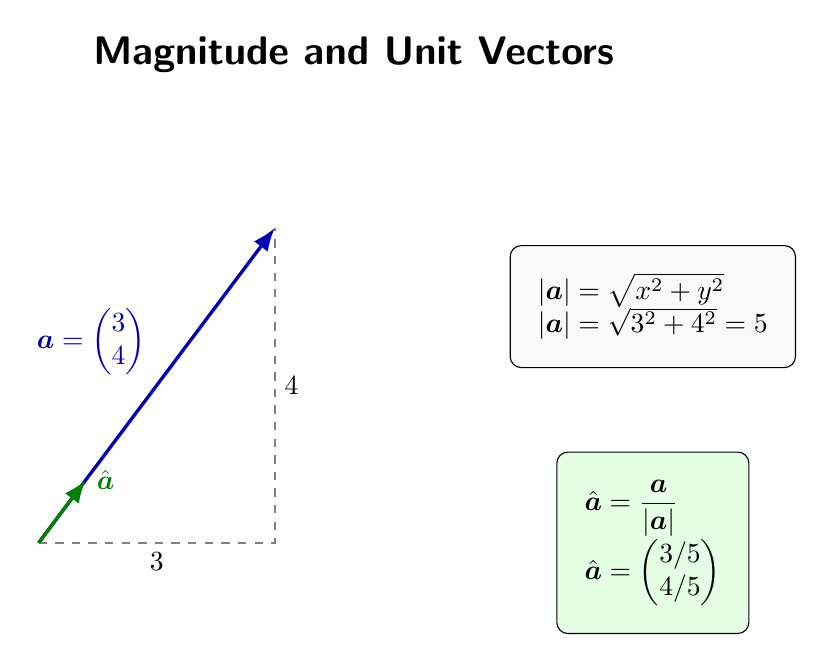
\begin{tikzpicture}[>=Latex,every node/.style={font=\sffamily},vector/.style={->,very thick,blue!70!black},unit/.style={->,very thick,green!50!black}]
\node[font=\sffamily\bfseries\Large] at (0,4.2) {Magnitude and Unit Vectors};
\coordinate (O) at (-4,-2);\coordinate (A) at (-1,2);
\draw[vector] (O)--node[above left] {$\bm a=\begin{pmatrix}3\\4\end{pmatrix}$}(A);
\draw[dashed,gray,thick] (O)--(-1,-2)--(A);
\node[below] at (-2.5,-2) {$3$};\node[right] at (-1,0) {$4$};
\draw[unit] (O)--(-3.4,-1.2) node[right] {$\hat{\bm a}$};
\node[draw,rounded corners,fill=gray!5,align=left,inner sep=10pt] at (3.8,1) {$|\bm a|=\sqrt{x^2+y^2}$\\$|\bm a|=\sqrt{3^2+4^2}=5$};
\node[draw,rounded corners,fill=green!10,align=left,inner sep=10pt] at (3.8,-2) {$\hat{\bm a}=\dfrac{\bm a}{|\bm a|}$\\$\hat{\bm a}=\begin{pmatrix}3/5\\4/5\end{pmatrix}$};
\end{tikzpicture}

\end{document}
